\section{Lecture 2}

\subsection{Rigid Body Transformations}
We begin with some basic definitions.
\begin{definition}[Point]
    In this class, a point $p \in \R^3$ is represented as:
    \[ p = \begin{bmatrix}
        p_x \\ p_y \\ p_z
    \end{bmatrix} \]
    where $x, y, z$ are some orthonormal axes that make a coordinate frame. In $\R^n$ we will write:
    \[ p = \begin{bmatrix}
        p_1 \\ p_2 \\ \vdots \\ p_n
    \end{bmatrix} \]
    The distance of the point from the origin is:
    \[ \norm{p} = \sqrt{p_1^2 + \dots + p_n^2} \]
\end{definition}

\begin{definition}[Vector]
    A vector $v \in \R^n$ is defined as the displacement between two points:
    \[ v = p - q = \begin{bmatrix}
        p_1 - q_1 \\ p_2 - q_2 \\ \vdots \\ p_n - q_n
    \end{bmatrix} = \begin{bmatrix}
        v_1 \\ v_2 \\ \vdots \\ v_n
    \end{bmatrix}\]
    The norm of the vector is defined the same way.
\end{definition}

\begin{definition}[Matrix]
    A matrix $A \in \R^{n \times m}$ is a $n$-by-$m$ array of real numbers.
\end{definition}

Now we define how point-mass motion functions. First, there is some $p(0) = \begin{bmatrix}
    x(0) & y(0) & z(0)
\end{bmatrix}^T$. Then, from this, we can get $p(t)$, its position at time $t$.
We define the "trajectory" of an object as this map from time to position.

Think about a "rigid body" like your cell-phone.

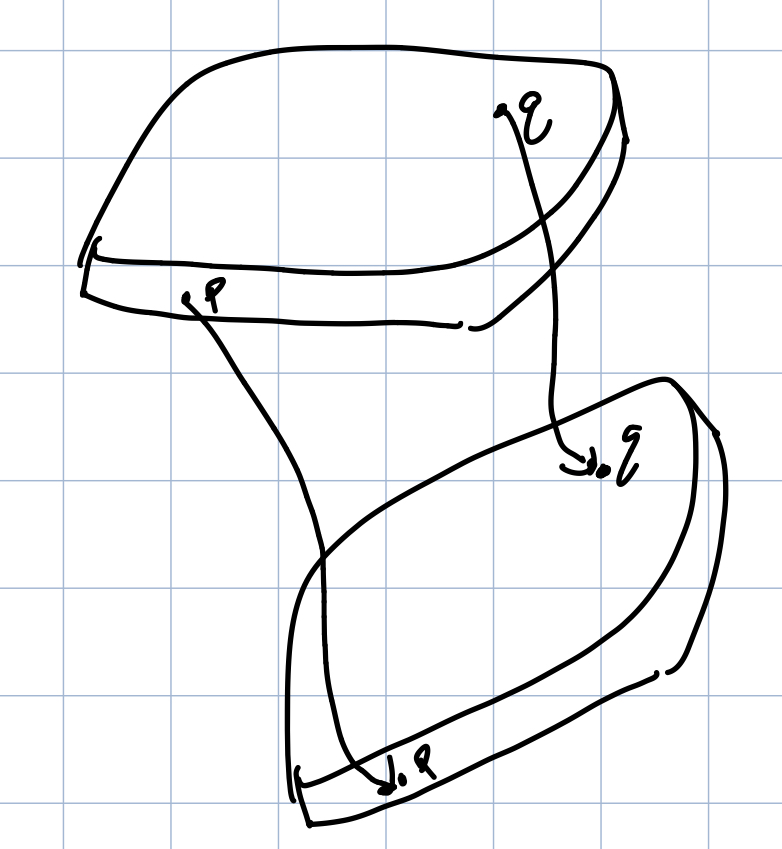
\includegraphics[width=300px]{rigidbody.jpeg}

As you move this rigid body,
if you take two points on the rigid body, their distance does not change.
\[ \norm{p(t) - q(t)} = \norm{p(0) - q(0)} = \text{constant}\]
i.e. the size of the vector between them stays the same. Furthermore, orientations stay the same. This leads to the following definition:

\begin{definition}[Rigid Body Transformation]
    A rigid body transformation is a function $g$ that has its domain as the set of all
    vectors in $R^3$ such that:
    \begin{itemize}
        \item Length (of vectors) is preserved.
        \[ \norm{g(p) - g(q) } = \norm{p - q} \]
        \item Orientation is preserved
        \[ g_{*}(v \cross w) = g_{*}(v) \cross g_{*}(w) \]
    \end{itemize}
    We use $*$ to denote $g$ operating on a vector rather than a point.
\end{definition}

\subsection{Rotational Motion in $\R^3$}

So the first step of modeling rotation is to choose a spatial reference frame $A$.
Then, we must attach a frame $B$ to the body.

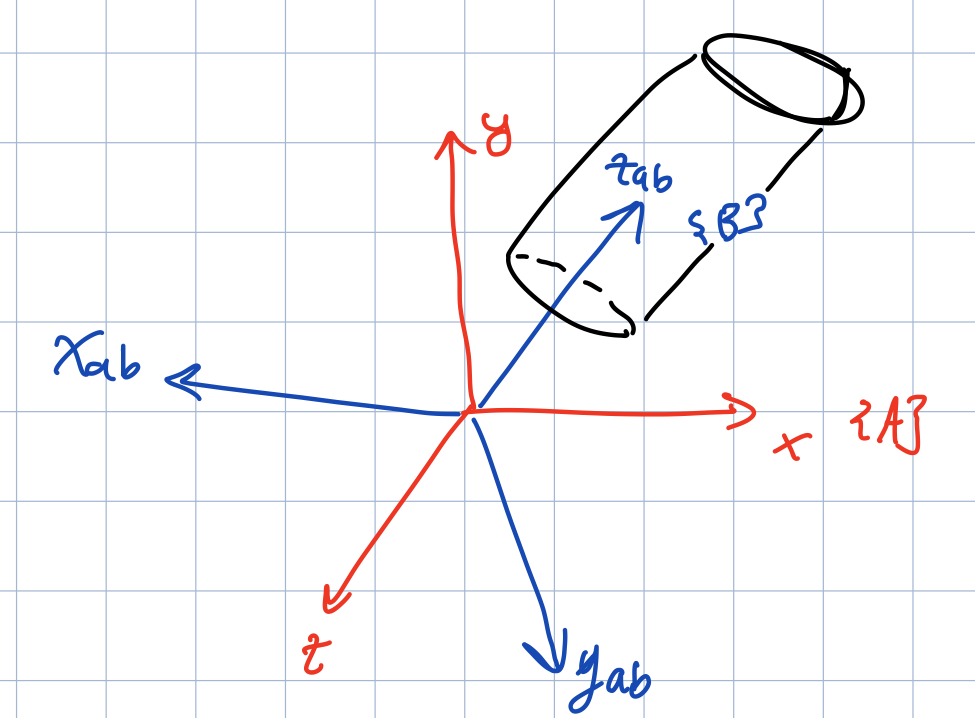
\includegraphics[width=300px]{rot.jpeg}

where $x_{ab} \in \R^3$ is the coordinates of $x_b$ in frame $A$.
\begin{definition}[Rotation Matrix]
    The rotation (or orientation) matrix of $B$ with respect to $A$ is defined as:
    \[ R_{ab} = \begin{bmatrix}
        x_{ab} & y_{ab} & z_{ab}
    \end{bmatrix} \]
\end{definition}

For any rotation matrix, the columns are orthonormal, i.e.
\[ r_i^T \cdot r_j = \begin{cases}
    0 & i \neq j \\
    1 & i = j
\end{cases} \]
which means $R$ is orthogonal, meaning it is in the set $O^{(3)}$.
\[ R \in O(3) \implies R^{T} R = R R^{T} = I \]

What is the determinant of $R$?
\[ \det(R^T R) = \det R^T \cdot \det R = (\det R)^2 = 1 \implies \det R = \pm 1 \]
However, if $R$ is a rotation matrix, $\det(R)$ must be 1. Why?
\[ det R = r_1^T(r_2 \times r_3) = 1 \]
Since $r_2 \times r_3 = r_1$ in a right-handed coordinate system.

\begin{definition}[SO($n$)]
    The special orthogonal group SO(3) is
    \[ R \in \R^{3 \times 3} \mid RR^T = R^TR = I, \det(R) = 1 \]

    This can be extrapolated to $n$ dimensions, SO($n$):
    \[ R \in \R^{n \times n} \mid RR^T = R^TR = I, \det(R) = 1 \]
\end{definition}

We used this term group, which is a mathematical object.

\begin{definition}[Groups]
    A group is a set $G$ requipped with by a binary operator $\cdot$ which satisfies
    \begin{itemize}
        \item The binary operation maps back onto the set itself (closure).
        \item The binary operation is associative ($g_1 \cdot (g_2 \cdot g_3) = (g_1 \cdot g_2) \cdot g_3$)
        \item There is a unique identity element such that $g \cdot e = e \cdot g = g$
        \item There is a unique inverse for every element such that $g \cdot g^{-1} = e$
    \end{itemize}
\end{definition}

Here are some examples of groups.
\begin{example}
    Here are some groups and non groups:
    \begin{itemize}
        \item $(\R^3, +)$
        \item $(\{0, 1\}, + \mod 2)$
        \item $(\R, \times)$ is NOT a group
        \item $(SO(3), \cdot)$
    \end{itemize}
\end{example}

It turns out $SO(3)$ (equipped with matrix multiplication) IS a group! Let's prove this.
\begin{proof}
    Consdier $R_1, R_2 \in SO(3)$. Then 
    \[ (R_1 R_2)^T (R_1 R_2) = R_2^T R_1^T R_1 R_2 = I\]
    and
    \[ \det(R_1 R_2) = \det(R_1) \det(R_2) = 1 \cdot 1 = 1 \]
    so therefore $R_1 \cdot R_2$. The identity element is the identity matrix,
    to take inverses you just transpose, and associativity comes for free from matrix multiplication properties.
    Thus, $SO(3)$ is a group.
\end{proof}

Now we are ready to dive into how rotations actually function. Consider a point $q$ and its coordinates in $B$:
$q_b = \begin{bmatrix}
    x_b & y_b & z_b
\end{bmatrix}^T$. Now to derive its coordinates in $a$, we simply realize:
\[ q_a = x_{ab} x_b + y_{ab} y_b + z_{ab} z_b = R_{ab} q_b \]

Finally, let us show rotations are a rigid body transformation. First we need to
define the skew symmetric part of a vector.

\begin{definition}[Skew Symmetry]
    A matrix $A$ is skew symmetric if $A^T = - A$. We denote the set of all skew symmetric matrices in $\R^3$ is
    $so(3)$.
\end{definition}

\begin{definition}[Skew Symmetric Part]
    The skew-symmetric part of a vector $a = \begin{bmatrix}
        a_1 & a_2 & a_3
    \end{bmatrix}^T$ is:
    \[ \hat{a} = \begin{bmatrix}
        0 & -a_3  & a_2 \\
        a_3 & 0 & -a_1 \\
        -a_2 & a_1 & 0
    \end{bmatrix} \]
\end{definition}

Now we can see the following:
\[ a \times b = \hat{a} b \]

Note that also:
\begin{theorem}
    We have the following cross product identities:
    \begin{itemize}
        \item Scalar triple product
        \[ a \cdot (b \cross c) = c \cdot (a \cross b) = b \cdot (c \cross a) \]
        \item Vector triple product
        \[ a \cross (b \cross c) = (a \cdot c) b - (a \cdot b) c \]
        \item Jacobi Identity
        \[ (a \cross b) \cross c + (c \cross a) \cross b + (b \cross c) \cross a = 0 \]
    \end{itemize}
\end{theorem}

These convenient facts come in handy, now we can prove that $R$ preserves distance and orientation, showing it is a rigid transformation:
\begin{proof}
    Consider two points $p_1, p_2$,
    \begin{align*}
        \norm{R p_1 - R p_2}^2 &= \norm{R (p_1 - p_2)}^2 \\
        \norm{R p_1 - R p_2}^2 &= (p_1 - p_2)^T R^T R (p_1 - p_2) \\
        \norm{R p_1 - R p_2}^2 &= (p_1 - p_2)^T (p_1 - p_2) \\
        \norm{R p_1 - R p_2}^2 &= \norm{p_1 - p_2}^2 \\
    \end{align*}
    so the norm does not change.

    Now consider two vectors $v$ and $w$:
    \begin{align*}
        R (v \times w) &= R \hat{v} w \\
        &= R \hat{v} R^T Rw 
    \end{align*}
    We claim $\hat{Rv} = R \hat{v} R^T$, which will complete the proof. To show this, suppose the rows of $R$ are $r_i^T$. Then:
    \begin{align*}
        \hat{Rv} &= \hat{\begin{bmatrix}
            r_1^T \\ r_2^T \\ r_3^T
        \end{bmatrix} v} \\
        &= \hat{\begin{bmatrix}
            r_1^T v \\ r_2^T v \\ r_3^T v
        \end{bmatrix}} \\
    \end{align*}
    But the other side is:
    \begin{align*}
        R \hat{v} R^T &= R \begin{bmatrix}
            \hat{v} r_1 \\ \hat{v} r_2 \\ \hat{v} r_3
        \end{bmatrix} \\
        &= \begin{bmatrix}
            r_1^T \hat{v} r_1 & r_1^T \hat{v} r_2 & r_1^T \hat{v} r_3 \\
            r_2^T \hat{v} r_1 & r_2^T \hat{v} r_2 & r_2^T \hat{v} r_3 \\
            r_3^T \hat{v} r_1 & r_3^T \hat{v} r_2 & r_3^T \hat{v} r_3
        \end{bmatrix}
    \end{align*}
    Where the $i, j$ component is:
    \[ r_i \cdot (v \times r_j) = v \cdot (r_i \times r_j) = \begin{cases}
        0 & i = j \\
        \text{the other dimension} & i < j \\
        \text{negative the other dimension} & i > j
    \end{cases}\]
    Note this is exactly the entries of the RHS, so we are done.
\end{proof}